\chapter{力の法則}

{\small 注: 数学リメディアル教材の第1・第2章を習得しておくこと。}

\section{力とは何か?}

小学校以来, 理科には何回も「力」が出てきたが, 諸君は「力」とは何か, わかっているだろうか?

「力」は, 有名な国語辞典である「広辞苑」(第六版電子版)では以下のように記されている:\\
(1) 自らの体や他の物を動かし得る, 筋肉の働き。(後略)\\
(2) 気力。精神力。根気。(後略)\\
(3) 能力。力量。実力。(後略)\\
...\\
(8) [理] 静止している物体に運動を起こし, また, 動いている物体の速度を変えようとする作用。(後略)\\

科学でいうところの「力」は, この(8)である。(1), (2), (3)とは全く
違うものである。

ところが, このことをきちんと理解せずに, 「力」を(1), (2), (3)のような
意味とごっちゃにして「理解」している人が多い。おそらく, 「物理が苦手」
「物理は嫌い」という人の多くがそうだろう。日常で使われる
(1), (2), (3)のイメージに引きずられて, ついつい「わかった気」に
なってしまっているのである。

余談だが, 力とエネルギーを混同している人も多い。後述するが, 
力とエネルギーは, 明確に別物である。「エネルギー」も日常でよく
出てくるので, なんか「わかった気」になってしまうのだろう。

科学では, このように, 「言葉にこだわる」姿勢が重要である。言葉に関する
間違った思い込みやあやふやな理解が, 理解を妨げるのである。

さて, 「広辞苑の(8)の説明を読んでもよくわからない」という人もいるだろう。
当然である。これを理解するには, 「運動」とか「速度」などを定義する必要
があるし, いろんな事例や観点について考えて納得していく必要があるからだ。

実は, この広辞苑の(8)は, 次章で詳述する「慣性の法則」と「運動方程式」を, 
部分的に言い換えたものである。これらの法則をもとに, 「力」が定義されるのだ。

「運動方程式」は, 数学リメディアル教材にも出てきたが, ざっくりいうと, 
力は質量と加速度の積に等しい, という法則である。その「意味」は次章で学ぶが, 
とりあえず, このことから力の「単位」がはっきりする。すなわち, SI単位系
では(SI単位系がわからない人はネットで検索するか, 「数学リメディアル教材」を
参照せよ), 質量の単位はkg, 加速度の単位はm~s$^{-2}$を使うので, 
その積は, kg~m~s$^{-2}$となる。これが, SI単位系における力の単位である。
これをN (ニュートン)\index{にゅーとん@ニュートン}と呼ぶ。
すなわち, 1~N=1~kg~m~s$^{-2}$である。

\begin{faq} {\small\textgt{力って, 本当に存在するのですか? 
目に見えないのでイマイチわかりません} ... 力というものが「本当に存在するかどうか」
は, 実はどうでもよいのです。「力」が実在すると考えれば, 宇宙の法則が矛盾なく簡潔に
整理できるのです。それが「力」の実在性の保証です。「そう考えれば全てつじつまが合う」
というのが, 物理学で認められる説得力であり, 正しさであり, 実在性なのです。
}\end{faq}

\begin{faq}{\small\textgt{結局, 「力」って何ですか?}
... あえて短く言えば, 物体の運動状態に変化をもたらすもの。}\end{faq}

\begin{faq}{\small\textgt{N (ニュートン)の定義がわかったようなわからないような...}
... kg~m~s$^{-2}$です。それ以外の何ものでもない。}\end{faq}
\mv

\begin{q}\label{q:4forece}
君は, 今まで「力」をどのように理解・認識していたか? 科学的に正確に
理解していたと言えるか? そうであれば, それはどのようなきっかけで
そうなったか? 正確に理解してはいなかったなら, なぜそうだったのか?
\end{q}


\section{4つの力}

%2011.4.1 ヤマサキ 脚注を変更。「田中さんの例」はむしろわかりづらいと感じました…。
自然界にはさまざまな力が存在するが, 根源的には, それらは以下の4つからなる
ということが, 物理学者達の長い苦闘の末, 明らかになっている:
\begin{itemize}
\item 重力
\item 電磁気力
\item 強い力(核力など)
\item 弱い力(ベータ崩壊など)
\end{itemize}
その他の力, たとえば摩擦力やバネの力などは, いずれもこれらの力から派生するものだ。
言い換えると, どのような力も,元をたどればすべてこの4つの力で説明できるのだ。

我々の身近な現象に関与する力は, ほとんどが重力または電磁気力だ。
「強い力」「弱い力」は, 「重力」や「電磁気力」と同じように, 
これ自体で科学的な専門用語である。何かの基準よりも強い(または弱い)
力を指すのではない。「強い力」は原子核の中で陽子や中性子を
同居させる力であり, これがなければ物質(元素)は存在できない。

「弱い力」は, 原子核のベータ崩壊(陽子が陽電子とニュートリノを発して
中性子に変わることなど)のときに関与する。その例として, 原発事故で
漏れ出した放射性セシウム$^{137}$Csが放射性バリウム$^{137}$Ba
に変わる崩壊がある。また, 放射性炭素$^{14}$Cが窒素$^{14}$Nに
変わる崩壊もベータ崩壊である。これは過去の生物遺体の年代測定に使われる。

\begin{q}\label{q:4forece}
自然界に存在する, 根源的な4つの力とは何か?
\end{q}
\hv


\section{力の一般的な性質}

ここで, 力の一般的な性質について学んでおこう。ここで述べるのは, その力
の起源が重力であれ電磁気力であれ何であれ, 例外なく成り立つようなことだ。
なお, 以後しばらく, 「物体」は質点と同義語と考えて欲しい。物体の大きさや
形を考えねばならないときは, 逐次, そのように言及する。

\begin{itemize}
\item 力には, 大きさと向きがある。つまり, 力はベクトルである。
\item ベクトルの数学に基づいて, 複数の力を足し合わせたり, ひとつの力を
複数の力に分解して考えてもよい。特に, ある物体に複数の力が働く場合, 結果的
には, その物体には, それらの力をベクトルとして足し算したもの(合力)\index{ごうりょく@合力}のみが
働くと考えてよい。
\item 物体が静止している場合, その物体に働く力(合力)はゼロである
\footnote{逆は必ずしも成り立たないことに注意せよ。すなわち, 働く力が
ゼロであっても物体は静止しているとは限らない。\textgt{力が働かなくても物体は
動いていることができるのだ}。(詳しくは慣性の法則のところで述べる)}。これを「力のつりあい」 \index{ちからのつりあい@力のつりあい}という。
これは後に述べる「慣性の法則」の特殊な場合だ。
\item 2つの物体A, Bにおいて, AがBに力を働くとき, AはBから, 同じ大きさで
逆向きの力を受ける。これを「\textgt{作用・反作用の法則}」\index{さようはんさようのほうそく@作用・反作用の法則}という。
\end{itemize}
\mv
ではこれから, いくつかの具体的な力について学んでいく。\\



\section{重力}\index{じゅうりょく@重力}

重力とは, 質量を持つ物体に働く力である。万有引力ともいう。
質量$M$と質量$m$をそれぞれ持つ2つの質点が距離$r$だけ離れて
いれば, その間に, お互いが引っ張る向きの力が生じる。
%(図\ref{fig:gravity})
\begin{comment}
\begin{figure}[h]
    \centering
    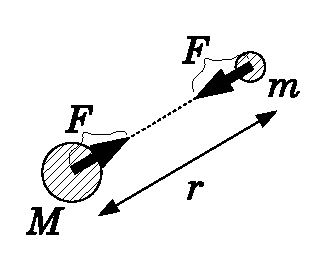
\includegraphics[width=5cm]{gravity.eps}
    \caption{2つの物体の間に働く重力。}\label{fig:gravity}
\end{figure}
\end{comment}
その力の大きさ$F$は以下の式を満たす:
\begin{itembox}{重力の法則}
\begin{eqnarray}
F=\frac{GMm}{r^2}\label{eq:gravity_univ}
\end{eqnarray}
\end{itembox}
これが重力だ。ここで, $G$は「万有引力定数」と呼ばれる定数で, 
\begin{eqnarray}
G=6.67\times 10^{-11}\text{ m}^3\text{ s}^{-2}\text{ kg}^{-1}
\end{eqnarray}
である。$G$の値は記憶しなくてもよいが, 式(\ref{eq:gravity_univ})は記憶せよ。

\eref{eq:gravity_univ}は, 英国の物理学者
アイザック・ニュートンが発見した。どうやって発見したのか? 
惑星の運行を説明するためにいろいろな数式を試行錯誤したのだ。ニュートンだけでなく, 
ガリレオ, ティコ・ブラーエ, ケプラー等の学者を含めた, 長い苦闘の成果である。

この式よりもさらに重力を一般的に説明する理論が「一般相対性理論」である。しかし
一般相対性理論は学類1年生には手に負えない理論なので, 我々は式(\ref{eq:gravity_univ})
を重力の基本法則(根源的な法則)とみなそう。\mv

ところで質量とはそもそも何だろうか? それは物体に重力を生じさせるような, 
物体の属性である。では重力とは何か? それは質量を持つ物体どうしに働く力だ。
この議論は循環論法だ。質量を定義するのに重力の概念が必要で, 
重力を定義するのに質量の概念が必要だ! こうして見ると, 世の中は
全てが論理的にすっきり説明できるものではなく, どこかで「そういうものが
あるのだ」と認めねば話がはじまらない。というわけで, 物体を特徴づける
量として質量というものが存在する, ということを天下りに認めよう。\mv

作用・反作用の法則のために, 質量$M$の物体が質量$m$の物体を引く力と, 
その逆, つまり質量$m$の物体が質量$M$の物体を引く力は, 互いに向きは逆だが, 
大きさは同じだ。質量の大きな物体が質量の小さな物体を引く力は, 
質量の小さな物体が質量の大きな物体を引く力と同じ大きさなのだ。

さて, 重力が最も活躍するのは, 天体の現象だ。星は, 重力に
よって物を引きつける。地球を含めて球状の星は, 重力に関しては, 
その中心に質量が集中しているとみなして扱える。例えば地球の
表面に立つ質量$m$の君に地球が及ぼす重力を考えるとき, 
$M$として地球の質量を, $r$として地球の半径を考えればよい。
これは自明なことではなく, 重力の法則をもとに数学的に証明
されることだが, ここではその詳細は述べない。気になる〜という
人は, まず大学の数学をしっかり勉強しよう。\mv

\begin{q}\label{q:grav_accel}
地球の半径を$r=6400$ km, 
地球の質量を$M=6.0×10^{24}$~kgとする。地表において質量$m=1.0$~kgの物体が受ける, 地球から
の重力が, 9.8 Nであることを示せ(有効数字二桁でよい)。ヒント: 単位を埋め込んで計算しないと
失敗するだろう!
\end{q}
\mv

\begin{comment}
ところで, 力はベクトル(大きさと向きを持つ量)\index{べくとる@ベクトル}なのだから, \eref{eq:gravity_univ}を, 
力の大きさだけでなく力の向きまできちんと表現できるような式に書き直すこともできる:
\begin{eqnarray}
{\mathbf F_{12}}=-\frac{G\,m_1 m_2({\mathbf r}_2-{\mathbf r}_1)}{|{\mathbf r}_2-{\mathbf r}_1|^3}\label{eq:gravity_univ_vect}
\end{eqnarray}
ここで, 2つの物体を, 物体1と物体2とし, ${\mathbf F_{12}}$は物体1が物体2に及ぼす重力(ベクトル), 
$m_1$, $m_2$はそれぞれ物体1と物体2の質量, ${\mathbf r}_1, {\mathbf r}_2$はそれぞれ物体1と物体2の
位置ベクトルである(大学ではベクトルを太字で書き表す)。
この式は, \eref{eq:gravity_univ}に「物体2から物体1へ向いた単位ベクトル」,すなわち
\begin{eqnarray}
-\frac{{\mathbf r}_2-{\mathbf r}_1}{|{\mathbf r}_2-{\mathbf r}_1|}
\end{eqnarray}
を付けた形になっている。\footnote{ベクトル${\mathbf r}_2-{\mathbf r}_1$(これは物体1を始点にして物体2まで伸びているベクトルである)を
そのベクトルの大きさ$|{\mathbf r}_2-{\mathbf r}_1|=r$で割って得られるベクトル(つまり${({\mathbf r}_2-{\mathbf r}_1)}/{|{\mathbf r}_2-{\mathbf r}_1|}$)が, 
「物体1から物体2へ向いた単位ベクトル」を表している。このベクトルをマイナス倍すると向きが逆になり, 結局この式は「物体2から物体1へ向いた単位ベクトル」を表すことになる。}
(図\ref{fig:gravity_vect})。
\begin{figure}[h]
    \centering
    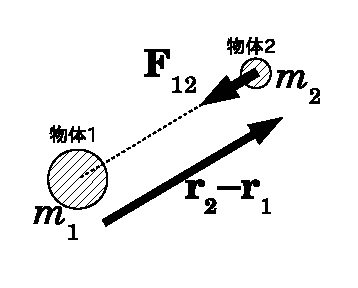
\includegraphics[width=5cm]{gravity_vect.eps}
    \caption{物体1が物体2に及ぼす重力${\bf F}_{12}$。}\label{fig:gravity_vect}
\end{figure}
\end{comment}

地表にある物体が地球から受ける重力について, もう少し考えよう。
$m$を地表の物体の質量, $M$を地球の質量とする。
地球中心から地表までの距離(つまり地球半径)を$r$とする。
地表の物体が地球から受ける重力の大きさ$F$は, 
\eref{eq:gravity_univ}から, 
\begin{eqnarray}
F=\frac{GM}{r^2}m\label{eq:gravity000}
\end{eqnarray}
となる。ここで, 物体を地球上のいろんなところに持って行っても, 
$G$, $M$, $r$はそれぞれ一定値とみなせる($r$だけは, 
高い山の上などに持って行くと微妙に変わるが, それでも
その変化はわずかである)。従って, 上の式の
\begin{eqnarray}
\frac{GM}{r^2}
\end{eqnarray}
は(ほぼ)定数とみなすことができ, これを$g$と置こう。すると
\eref{eq:gravity000}は, 
\begin{eqnarray}
F=mg\label{eq:gravity_earth}
\end{eqnarray}
と書ける。このとき, 比例係数$g$を「\textgt{重力加速度}」
\index{じゅうりょくかそくど@重力加速度}と呼ぶ(記憶せよ)。

実は, 上の説明はあまり正確ではない。例えば地球の形は完全な球形では
なく, 赤道付近がわずかに膨らんだ, 楕円体である(だから, 地球の中心に
質量が集中しているとみなすのは, 厳密にはダメである)。また, 地球
の密度は均一でないために, 地表の場所によって重力は大きかったり
小さかったりする。さらに, 実際に地表で感じられる重力には, 後で学ぶ
「遠心力」(地球の自転に起因する力)も加わる。従って, 実際は$g$の
値は場所によって微妙に異なる。これは生物資源学類としては注意が
必要なポイントだ。

\begin{q}\label{q:weight_calib} 化学実験では, 
試薬を量り取る時に電子天秤を使う。
電子天秤で量る重さは, その場の重力加速度に比例する。北海道大学(札幌市)
と筑波大学で同じ電子天秤を調整せずに使ったら, 重さの測定値は何%くらい違うか?
ヒント: 「電子天秤の校正 札幌 茨城」などをキーワードにして
インターネットなどで調べよ。\end{q}

これを意識しないと, 北大と筑波大で同じ実験をしたつもりでも, 
試薬の量が異なってしまい, 違う実験結果になりかねない!\mv

さて, なぜ$g$の呼び方に「加速度」という言葉がついているだろう? それは, $g$の次元を
考えればわかる。まず, \eref{eq:gravity_earth}より, $g=F/m$である。一方, 
さきほど学んだように, 
$F$のSI単位はN(ニュートン; kg~m~s$^{-2}$), $m$のSI単位はkgなので, $g$すなわち$F/m$
のSI単位は, kg~m~s$^{-2}$/kg = m~s$^{-2}$。従って, $g$は, 
加速度の次元を持つのだ。実際, 問\ref{q:grav_accel}の結果から, 
$m=1.0$~kgのとき$F=9.8$ Nだったので, 
$g=F/m$を計算すれば, 
\begin{eqnarray}
g= 9.8\,\,\text{m~s$^{-2}$}
\end{eqnarray}
である(この値は記憶せよ)。

ここでは$g$が加速度の次元を持つことを示したが, $g$は実際に加速度として
意味を持っている。君が地表付近で何かの物体を落としたら, その物体はほぼ
一定の加速度$g$で加速しながら落下するのだ。そのあたりの事情は, 後で詳しく述べる。

% ジオイド, 遠心力, はかりの校正

\begin{q}\label{q:what_is_g}
重力加速度とは何か?
\end{q}
\mv

\begin{q}\label{q:geostat_sat}
高度10,000~mの上空を飛ぶ旅客機と, 高度36,000~kmの上空を飛ぶ静止衛星には, 
それぞれ地表での重力の何パーセントの重力がかかるか? ヒント:
式(\ref{eq:gravity_univ})を使う。それぞれの$r$は地表での$r$の何倍になるか?
\end{q}
\mv

\begin{q}\label{q:moon_gravity}
月の質量は地球の質量の1/81.3, 月の半径は地球の半径の1/3.68である。月の表面で, 
月から受ける重力は, 地球の表面で, 地球から受ける重力の何倍か?
ヒント:式(\ref{eq:gravity_univ})を使う。$M$と$r$の両方が変わることに注意。
\end{q}
\mv

%\begin{q}\label{q:atm_pressure}
%地表での平均的な大気圧は, 1000 hPa程度である。1.0~m$^2$の地表面の上空には, 
%どのくらいの質量の大気が存在するか?
%ヒント:式(\ref{eq:gravity_earth})を使う。1.0~m$^2$の地表面の上空にある大気の
%質量を$m$とすれば, それにかかる重力$mg$が, 地表面での圧力を生む。なお重力は
%厳密には高さによって変わるが, ここではその変化を無視してよい。
%\end{q}\mv

\begin{faq}{\small\textgt{地球の中心に行けたら, 万有引力はどのように働くのでしょうか?}
... 全方向からの引力が打ち消しあって0になります。要するに「無重力」です。}\end{faq}\mv

\begin{faq}{\small\textgt{地球の質量は一定ですか? いろんな反応が
起こって絶えず変わっているイメージです。}
... 地球には隕石等が宇宙から飛来して質量を増やす一方, 地球大気から(地球の重力を
ふりきって)宇宙に飛散する分子や原子もあり, 質量を減らす。そんなこんなで, 地球の質量は, 
絶えず微妙に増減しているでしょう。}\end{faq}\mv

\begin{faq}{\small\textgt{万有引力はどんな物体の間にも
はたらいているのですか?例えば人と人の間とか。}
... 質量を持つ物体ならどんな物体の間にも働いています。もちろん人と人の間にも働いていますよ。}\end{faq}
\hv



\section{クーロン力}\label{sect:CoulombForce}\index{くーろんりょく@クーロン力}
次に, 電磁気力について考えよう。電磁気力とは, 「電荷」を
持つ物体に働く力のことだ。

物質を構成するのは原子核や原子, イオンなどであり, それらを構成するのは, 
電子や陽子, 中性子, 中間子など, 「素粒子」と呼ばれる微細な粒子だ。
なぜだかわからないが, それぞれの素粒子には, \underline{電荷}
\index{でんか@電荷}という, 固有の性質(物理量)がある。
電荷の性質として, 
\begin{itemize}
\item 電荷は正と負という符号のある量である。
\item 電子1個と陽子1個は, 同じ大きさで逆の符号の電荷を持っている。
\end{itemize}
ということが知られている。これらがなぜなのかは, 根本的には
わかっていない。そのようにこの世界は作られているのだとしか
言う他はない。そして, 電子1個や陽子1個が持つ電荷の大きさを
$1.602\times 10^{-19}$~Cとする(Cというのは電荷の単位であり, 
「クーロン」と呼ぶ。SI基本単位で表せば, 1 C=1 A~sだ)。
これを\underline{電荷素量}\index{でんかそりょう@電荷素量}と呼び, 
$q_e$とあらわす。$q_e$は, 有効数字4桁では, 
$q_e=1.602\times10^{-19}\text{ C}$である(記憶せよ)。
電子の電荷を$-q_e=-1.602\times10^{-19}\text{ C}$, 
陽子の電荷を$+q_e=1.602\times10^{-19}\text{ C}$とする。

原子核や原子, イオン, 分子などの粒子や, もっと大きい物体は, 
それを構成する素粒子の持つ電荷の総和(正の値と負の値を加えて
差し引きした量)を電荷として持つ, と約束する。例えば, 
水素原子は1個の陽子と1個の電子から構成されるが, 陽子と
電子の電荷は同じ大きさで逆符号なので, その総和は0である。
従って, 水素原子の持つ電荷は0である, とみなす。正の電荷
と負の電荷のどちらかが多いときだけ, その粒子は0以外の
電荷を持つことになる。粒子や物体が0以外の電荷を持つときは, 
その粒子や物体は「帯電している」という。帯電している粒子の
ことを荷電粒子という。電子や陽子, 原子核, イオンなどは
荷電粒子だ。荷電粒子のことを電荷ということもある。\mv

さて, 電磁気力のひとつを紹介しよう。「粒子1」と「粒子2」という2つの荷電粒子がある
とき, それらの間には, 電荷に応じて, お互いを引っぱる
向きの力(引力)またはお互いを遠ざける向きの力(斥力)が働く。その引力または
斥力の大きさを$F$とすると, $F$は以下の式を満たす:
\begin{itembox}{クーロンの法則}\index{くーろんのほうそく@クーロンの法則}
\begin{eqnarray}
F=\frac{k\,q_1\,q_2}{r^2}\label{eq:coulomb}
\end{eqnarray}
\end{itembox}
ここで, $q_1, q_2$は粒子1と粒子2がそれぞれ持つ電荷, $r$は粒子間の距離である。
$k$は定数で, 有効数字4桁では, $k=8.987\times 10^{9}$ N~m$^2$ C$^{-2}$だ。
この式(\ref{eq:coulomb})を, クーロンの法則 (Coulomb's law)と呼び, このように
記述される電磁気力をクーロン力 (Coulomb force)と呼ぶ。クーロンというのは, この法則
を見つけた物理学者の名前だ。$k$の値は記憶しなくてもよいが, 式(\ref{eq:coulomb})
は記憶しよう。\mv

クーロン力は, 電荷を持つ物体に働く力だ。一方, 
重力は, 質量を持つ物体に働く力であった。興味深いことに, これらの
数学的な表記, すなわち\eref{eq:coulomb}と\eref{eq:gravity_univ}
は, 互いによく似ている。従って, 重力に関して成り立つ議論, 特にその数学的な扱いは, 
クーロン力にも通用することが多いし, その逆も然りである。

\begin{faq}{\small\textgt{性質も似ているのでしょうか? この2つの式は統合できるのでは?}
... 地球中心で重力がゼロになるように, 一様に帯電した球の中心では電場がゼロになる, などの, 
よく似た性質があります。しかし, これらの式の統合には, 誰も成功していません。}\end{faq}\mv

さて, 上述のように, 電荷には, \textgt{正電荷}と\textgt{負電荷}の二種類がある。$q_1$とか$q_2$は
プラスやマイナスの値をとり得るのだ。そして, $q_1$と$q_2$が同符号(両方ともプラス, 
もしくは両方ともマイナス)のとき, 式(\ref{eq:coulomb})から$F$はプラスになり, そのとき, 
2つの粒子の間には, 斥力(互いに遠ざける力)がはたらく。一方, $q_1$と$q_2$が異符号
(片方がプラスで片方がマイナス)のとき, $F$はマイナスになる。力の大きさがマイナスに
なるのは奇妙だが, このマイナスは, 2つの粒子の間に, 引力(互いに引き合う力)が
はたらくことを意味する (ここが重力との大きな違いだ。重力には
引力しかない。また,質量にはプラス(またはゼロ)しかない)。つまり, 
\eref{eq:coulomb}は力の大きさだけでなく向き(引力か斥力か)も表現している。

\begin{comment}
このあたり
の事情も考慮して, \eref{eq:coulomb}を, きちんと力の向きまで完全に記述できる
ように書くと, 次式のようになる:
\begin{eqnarray}
{\mathbf F_{12}}=k\,\frac{q_1 q_2({\mathbf r}_2-{\mathbf r}_1)}{|{\mathbf r}_2-{\mathbf r}_1|^3}\label{eq:coulomb_vect}
\end{eqnarray}
%2011.4.2 ヤマサキ 「ベクトルで表した重力の式についての変更」と連動して変更。
ここで, ${\mathbf F_{12}}$は粒子1が粒子2に及ぼす力(ベクトル), ${\mathbf r}_1, {\mathbf r}_2$はそれぞれ
粒子1と粒子2の位置ベクトルである。
このような式の形になる理由は, 重力のとき(\eref{eq:gravity_univ_vect})の事情と同様だ。\mv

\begin{faq}{\small\textgt{なぜ$q_1q_2<0$のとき${\bf F}_{12}$は引力で, 
$q_1q_2>0$のとき${\bf F}_{12}$は斥力になるのですか?}
... \eref{eq:coulomb_vect}を見ると, ベクトル${\bf F}_{12}$が, 
ベクトル${\mathbf r}_2-{\mathbf r}_1$を何倍かした形になっています。
その係数$k\,q_1\,q_2/|{\mathbf r}_2-{\mathbf r}_1|^3$の正負
は$q_1q_2$の正負で決まります。これが正のときは, ${\bf F}_{12}$は
${\mathbf r}_2-{\mathbf r}_1$と同じ向き, すなわち粒子1から粒子2までの
ベクトルと同じ向きです。すなわち, 粒子1が粒子2に及ぼす力は, 粒子2を
押しのける方向に働く, というわけです。$q_1q_2<0$のときはその逆。}\end{faq}
\end{comment}

\begin{q}\label{q:coulomb_law}
クーロンの法則とは何か?
\end{q}
\mv

\begin{q}\label{q:element_charge}
電荷素量とは何か?
\end{q}
\mv

\begin{q}\label{q:elec_grav_compare}
互いに1.0~m離れたところに存在する2個の電子の間には, 
クーロン力と重力の両方が働く。そのクーロン力を$F_e$, 重力を$F_g$とする。
\begin{enumerate}
\item $F_e$の大きさを求めよ。
\item $F_g$の大きさを求めよ。ただし, 電子の質量$m_e$は, $9.1\times10^{−31}$~kgである。
\item $F_g$は$F_e$の何倍か?
\end{enumerate}
\end{q}\mv


\section{電場と磁場}

さて, 電磁気力には, クーロン力だけでなく, 磁気的な力(磁力)もある。
クーロン力は, 荷電粒子が静止していようが運動していようが, 
無関係に働く。ところが磁力は, 荷電粒子が運動しているときにのみ働く。
それらを含めて正確に言えば, 次のようになる(今は詳細は理解しなくてよい):

電磁気力とは, 荷電粒子の電荷$q$に比例するような力であり, それは何らか
の2つのベクトル${\bf E}$, ${\bf B}$を用いて, 
\begin{eqnarray}
{\bf F}=q{\bf E}+q{\bf v}\times{\bf B}\label{eq:LorentsForce}
\end{eqnarray}
と書けることがわかっている(${\bf v}$は荷電粒子の速度)。
このような形で荷電粒子に力を及ぼすようなベクトル${\bf E}$
と${\bf B}$を, それぞれ\underline{電場}\index{でんば@電場}
と\underline{磁束密度}\index{じそくみつど@磁束密度}
と呼ぶ(定義)。

ここで$\times$という記号が出てきた。これはただの掛け算ではなく, 
ベクトルの「外積」というものである。今はこれは理解できなくてもよい
(知りたい人は数学リメディアル教材を参照)。「そんなものがあるのか」
という程度の理解でOK。そして, ある定数を磁束密度にかけたものを
\underline{磁場}\index{じば@磁場}という(詳細は割愛する)。\mv

電場と磁場は不可分であり, 互いに影響を及ぼしあうから, これらを
まとめて語るのだ。その基本法則を「マクスウェル方程式」という。これは本書では
扱わない。それを理解するには, 「ベクトル解析」\index{べくとるかいせき@ベクトル解析}
という高度な数学(ベクトルの微分と積分に関する数学)が必要であり, 
今の君には難しい。また, 特殊相対性理論というものでは, 
電場と磁場が統一されるのだが, それも難しすぎるので
本書では学ばない。\mv

\begin{q}\label{q:Coulomb_EF} 1個の電子から1.0~mの距離にある点
での電場の大きさを求めよ。ヒント: 今は${\bf B}$を考えなくてよい。\end{q}\mv

\begin{faq}{\small\textgt{高校で磁力を習った時, フレミングの左手の法則
というのがありましたが...}
... \eref{eq:LorentsForce}があればフレミングの左手の法則は不要
です。
\eref{eq:LorentsForce}はフレミングの左手の法則を包含し, それよりも
一般性の高い, 強い式なのです。ただしこれを使いこなすには「外積」を
理解する必要があります。がんばって数学を勉強してください!}\end{faq}

\begin{faq}{\small\textgt{磁力は電荷を持った粒子が運動しているときに働く
とのことですが, 静止した磁石同士にはたらく磁力はどうなんですか?}
... 磁石の中では電子のスピンというもののせいで, 電流が流れているのです。
それに磁力がかかるのです。}\end{faq}

\begin{faq}{\small\textgt{「今は理解できなくてよい」のなら, ここで教えなくても
いいんじゃないですか?}
... 「そんな言葉を聞いたことがある」「そんな式を見たことがある」
というのが大事なのです。そういうのが「伏線」になり, 皆さんの学習効率
を高めるのです。}\end{faq}\mv


\section{張力}
ここまでは, 上で述べた根源的な4つの力について学んだ。
ここからは, この4つの力から派生する力について学ぼう。
まずは「張力」という力だ。

例として, 君が天井から垂れ下がったロープに吊り下がって静止しているとしよう
(簡単のため, ロープの質量は無視する)。
ロープに1箇所でも弱い部分があればロープは切れて君は落下するだろう。従って, 
君に働く重力は, ロープの全ての箇所にも働いていることがわかる。
\begin{figure}[h]
    \centering
    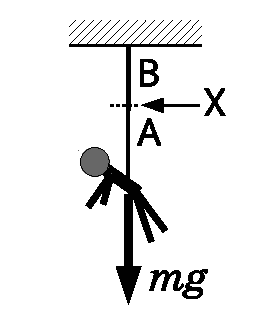
\includegraphics[width=5cm]{string.eps}
    \caption{ロープに吊り下がる人}\label{fig:string}
\end{figure}

ではロープの任意の1箇所Xを考えよう。そこより下の部分をロープA, そこより上の部分を
ロープBと呼ぼう。本来はロープAとロープBはXで繋がっていて1本のロープなのだが, 
便宜上, そう名づける。

さて, ロープAはロープBを下向きに引っ張っている。これは直感的に明らかだ。
一方, 同時にロープBはロープAを上向きに引っ張っている。
これは作用・反作用の法則に従えば明らかである(ロープAを「物体A」, ロープBを「物体B」として考えればよい)。
ロープBがロープAを上向きに引っ張っているというのがわかりにくければ, 次のように考えてもいい:
仮にロープBがロープAを上向きに引っ張っていないとすると, 
「君の体とロープAを合わせた物体」に働く力は重力のみである。しかし今, 
「君の体とロープAを合わせた物体」はロープに吊られて「静止」している。
静止しているからには, 「力のつりあい」が成り立たなくてはならない。
従って, ロープBはXにおいてロープAに「君に働く重力と同じ大きさで, 反対向き(上向き)の力」
を及ぼしていると考えざるを得ない。

これらの考察の結論(「君に働く重力と同じ大きさの力は, ロープの任意の箇所(つまり全ての箇所)
にも働いている」「ロープの任意の箇所では, そこを挟んで互いに逆向きで同じ大きさの力が働いている」)から, 
次のような結論が得られる: すなわち, ロープの端に力が働く場合, それと同じ大きさの力が, 
ロープの任意の箇所において, その箇所を挟んで互いに逆向きに働く。

このような力を\textgt{張力}と呼び, 慣習的に$T$で表す。張力には以下のような性質がある
(というか, 以下が張力の定義である):
\begin{itemize}
\item 張力は糸状の物体(ロープなど)に働く。
\item 張力は糸の各箇所で, 糸(の接線)に平行に働く。
\item 糸にかかる摩擦力や, 糸自体の質量にかかる重力が無視できる限り, 張力の大きさは糸のどこでも同じである。
\item 張力は, 引っ張りの向きにしか働かない。つまり, 糸を任意の箇所で2つに分割すると, 両者は互いに引き合う
力を及ぼす(互いに押し合う力は及ぼさない)。
\end{itemize}

ところで, 不幸にしてXが弱かったらどうなるだろう? ロープはXで重力に耐えきれずに, 次第に伸びて, 最後には切断されてしまう。
そうなると, 君に働く重力に抗っていた力は消えてしまい, 君は落下してしまうことになる。
ただし, その場合でも, ロープが完全に切断される寸前まで張力は存在するのだ。

\begin{q}\label{q:force_rope1}
図\ref{fig:string2}のように, 片端が壁にとりつけられた綱を力$F$で引く場合(上)
と, 両端を力$F$で引く場合(下)では, 綱にかかる張力の大きさは, どちらも$F$で等しい。このことを
説明せよ。
\begin{figure}[h]
    \centering
    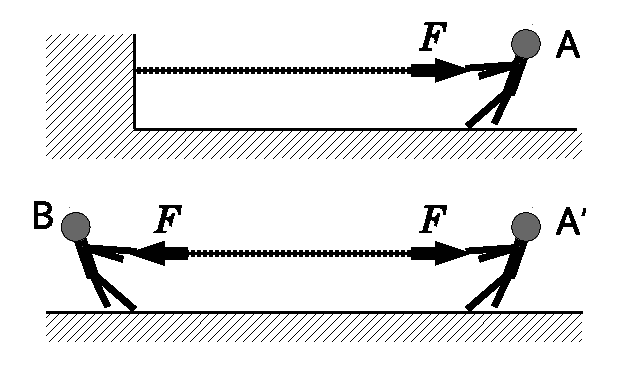
\includegraphics[width=7cm]{string2.eps}
    \caption{壁対人の綱引き(上)と, 人対人の綱引き(下)}\label{fig:string2}
\end{figure}
\end{q}

%
\begin{q}\label{q:force_rope3}
図\ref{fig:string3}のように, 質量$m$の君は, 天井に吊り下げられた滑車に
通されたロープの片端を体に結び, もう片端を手に持って, 自らの力で自らの体を
持ち上げようとしている。君の手がロープを引く力は$mg/2$であることを示せ(つまり, 
体重の半分の力で君は自分を持ち上げることができるのだ)。
\begin{figure}[h]
    \centering
    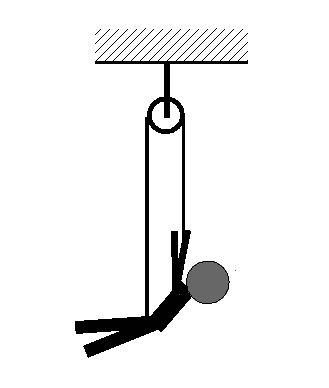
\includegraphics[width=4cm]{string3.eps}
    \caption{自力で上昇しようとする人}\label{fig:string3}
\end{figure}
\end{q}
\mv

%
\begin{q}\label{q:force_rope4}
図\ref{fig:string4}のように, 君は, 天井から固定された滑車Aと, 自由に
上下できる滑車B(動滑車)を利用して, 質量$m$の物体をロープで持ち上げようと
している。滑車の質量は無視し, ロープと滑車の間の摩擦は無いものとする。ロープは
一端が天井に固定され, 滑車Bと滑車Aを通って, もう一端が君の手に握られている。
君がロープを引っ張るのに必要な力は, 
$mg/2$であることを示せ。ヒント:ロープにかかる張力を$T$とすると, 滑車Bには上向き
に$2T$の力が働く。
\begin{figure}[h]
    \centering
    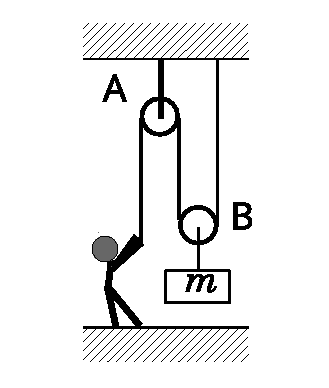
\includegraphics[width=5cm]{string4.eps}
    \caption{動滑車を使って物を持ち上げる}\label{fig:string4}
\end{figure}
\end{q}

\begin{faq}{\small\textgt{要するに天井と人が半分ずつ引っ張っているということ?}
... そうです。}\end{faq}\mv


問\ref{q:force_rope4}の考え方を援用すれば, 図\ref{fig:string4_iketeru}のように, 
動滑車の数を増やせば増やすほど, 小さな力で物を持ち上げることができる, ということがわかるだろう。
\begin{figure}[h]
    \centering
    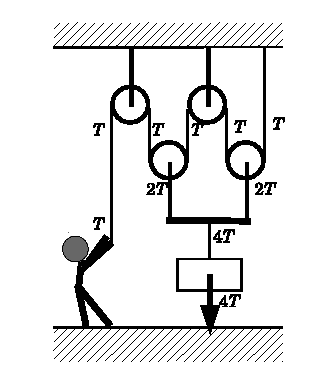
\includegraphics[width=6cm]{string4_iketeru.eps}
    \caption{2個の動滑車を使えば, 必要な力は1/4になる。}\label{fig:string4_iketeru}
\end{figure}

%
\begin{q}\label{q:force_rope5}
君の手がロープを引っ張るとき, その力の根源は何か?自然界に存在する4つの
根源的な力に帰着して説明せよ。
\end{q}
\hv



\section{圧力と応力}

化学などでは「圧力」\index{あつりょく@圧力}がよく出てくる。
圧力は, 面に垂直にかかる力を, 面積で割ったもの
(すなわち, 単位面積当たりの力)である。

圧力は, 「面に垂直」以外の方向まで含めて, 「面にかかる力を面積で割ったもの」
をあらわす時は, 「応力」\index{おうりょく@応力}という。圧力は応力の一種である。
特に, 面に平行にかかる力を面積で割ったものを, 「せんだん応力」という。それに
対して, 圧力のことを「垂直応力」ともいう。

当然ながら, 圧力や応力の単位は, 力の単位を面積の単位で割ったものである。
SI単位系では, N/m$^{2}$である。N=kg~m~s$^{-2}$なので, これはkg~m$^{-1}$~s$^{-2}$
とも書ける。この単位のことをPa (パスカル)と呼ぶ。

圧力は力ではない。圧力に面積を掛けたものが力である。

力はベクトルだが, 圧力は, 多くの場合, ベクトルでなくスカラーとして表現する。
その理由は, ここでは述べない。とりあえず「その方が便利だから」ということで
納得しておいてほしい。以下でも, 圧力やせん断応力はスカラーとして扱う。

\begin{exmpl} 底面積が$A=$0.50~m$^2$で質量が$m=$3.0~kgの箱がある。
この箱を地面に置いた時, 箱の直下の地面にかかる圧力を求めよう。

重力加速度を$g$とする。箱の重さは$mg$であり, これが地面にかかる力。
従って圧力は, $mg/A=3.0$~kg$\times 9.8$~m~s$^{-2}/$(0.50~m$^2)\fallingdotseq 60$~kg~m$^{-1}$~s$^{-2}\fallingdotseq 60$~Pa。(例おわり)
\end{exmpl}

\begin{q} 上の例で, 箱の質量はそのままで, 
箱の底面積が1/10になると(つまり0.050~m$^2$になると), 圧力はどうなるか?
\end{q}

\begin{q}\label{q:pressure_shoes} 君が立っている時, 君の足の裏の
直下の地面にはどのくらいの圧力がかかっているかを見積もれ。君の体重や
足の裏の面積などは適当な数値を仮定せよ(多少の嘘はOK)。
\end{q}

\begin{q}\label{q:pressure} 地表面での大気圧はおよそ1000~hPaである。
数学リメディアル教材で学んだように, hPaのhは「ヘクト」であり, 100を意味する。
\begin{enumerate}
\item 面積1~m$^2$の地表には, どのくらいの力がかかっているか?
\item 面積1~m$^2$の地表の真上には, どのくらいの質量の大気があるか?
\end{enumerate}
\end{q}

\begin{faq}{\small\textgt{人間が地上にいるとき, 大気の圧力に
押しつぶされないでいられるのは, どのような力が内側からはたらいて
いるのですか? また, もし人間が体ひとつで圧力のあまりかからない
ものすごく高い場所に行ったとしたら, その人は破裂するのでしょうか?}
... 人体の大部分は水であり, そもそも(液体の)水は圧力がかかってもあまり
変形しません。それが「つぶれない」ことのひとつの理由。また, 肺に空気がありますが, 
鼻を介して肺は外気とつながっているのでその圧力は基本的に外気の圧力(大気圧)と同じ。
従って, 肺の空気は大気圧と同じ圧力で押し返すから肺もつぶれない。ただし, 人間が
体ひとつで潜水する場合は, これが成り立ちません。特に, 水圧のために肺の空気が圧縮
されます。そのため, ある程度以上の深さに潜ると, 人間の体に働く浮力(それは体積に
比例する)が小さくなって, 人間の体は勝手に沈んでいくそうです(先日, テレビでやって
いました)。

逆に気圧の低いところ, 特に真空等に行ってしまうと, 体液が沸騰します(一般に, 
圧力が低くなると液体の沸点は下がる)。}\end{faq}
\mv


\section{弾性力(フックの法則)}

%2011.4.2 ヤマサキ 後に「バネの自然長」という言葉が使われているけど,それまでに説明がされてないので少し追加。
次に, バネについて考えてみよう。バネの自然状態での(力がかかってないときの)長さを「バネの自然長」と呼ぶことにする。
我々の日常経験から, バネを伸ばせば伸ばすほど強い力が働くことは自明だろう。
バネみたいに, 変形させると力を生じる物体について, 変形(変位)$x$と力$F$の関係を
関数$F(x)$で書くと, その関数がどんなものなのかはわからなくても, とりあえず
微分の定義から, 
\begin{eqnarray}F(x+dx)=F(x)+F'(x)dx\end{eqnarray}
となる($dx$は微小量)。ここで, $x=0$がつりあいの位置(バネの片端を固定し, 
自然状態に保ったときのもう片端の位置)に来るように座標を
とれば, $x=0$では力は働いていないから, $F(0)=0$となる(図\ref{fig:spring}の上の図)。
すると上の式は, 
\begin{eqnarray}
F(0+dx)&=&F(0)+F'(0)dx
\end{eqnarray}
つまり
\begin{eqnarray}
F(dx)&=&F'(0)dx
\end{eqnarray}
となる。この式は微小な量$dx$にしか厳密には成立しないけど, $x$が十分に小さい範囲に
限定して, $dx$を$x$と置き換えても近似的に成り立つと仮定すれば, 
\begin{eqnarray}
F(x)=F'(0)x\label{eq:HookeLaw3}
\end{eqnarray}
となる。ここで$F'(0)$の符号について考えてみよう。バネの力というものは, 伸ばせば
縮まる方向に, 縮めれば伸びる方向に働く。つまり, 変形(変位)と逆向きに働く。
従って, $x$が正なら$F$は負, $x$が負なら$F$は正である。従って, \eref{eq:HookeLaw3}に
おいて$F'(0)$は負であるはずだ。そこで, 形式的に$F'(0)$を$-k$と書き換えよう。このとき
$k$は正の定数である。すると\eref{eq:HookeLaw3}は, 
\begin{itembox}{フックの法則}
\begin{eqnarray}
F=-kx\label{eq:Hooke}
\end{eqnarray}
\end{itembox}
となる。ここで, $F$は, バネから受ける力, $x$はバネの伸び, $k$は\textgt{バネ定数}
\index{ばねていすう@バネ定数}と言われる定数である。これをフック(Hooke)の法則
\index{ふっくのほうそく@フックの法則}という。
\begin{figure}[h]
    \centering
    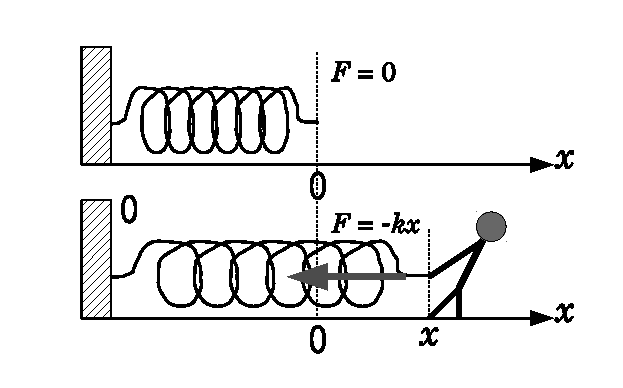
\includegraphics[width=8cm]{spring.eps}
    \caption{Hookeの法則}\label{fig:spring}
\end{figure}

このような数学的な考え方を線型近似と言う(数学リメディアル教材参照)。
要するに, フックの法則は, 力と変形(変位)の関数の線型近似式に過ぎず, バネ定数とは
その関数の微分係数(の絶対値)に過ぎない。

\eref{eq:Hooke}から明らかに, バネが伸びるほど力の大きさは大きくなる。繰り返すが, 
右辺のマイナスは, バネの伸びの方向($x$の符号)と力の方向($F$の符号)が逆だよ, 
ということを示す。バネは伸びると($x$が正だと), 縮もうとする力, つまりひっぱる
力を生じるから$F$は負になる。一方, バネは縮むと($x$が負だと), 伸びようとする力
を生じるから$F$は正になる。

\begin{q}\label{q:Hooke_law} 
\begin{enumerate}
\item フックの法則とは何か?
\item バネ定数とは何か?
\item バネ定数のSI単位は?
\end{enumerate}
\end{q}
\mv

さて, この「法則」は, 万有引力の法則やクーロンの法則よりも, ずっと一般性の
低い「しょぼい」法則である。フックの法則は, 限定的な例にしか成り立たない経験則
に過ぎない。実際, バネをどんどん伸ばすと, まっすぐな針金になってしまって, 
それ以上は伸びようがない。無理に伸ばすと, ぶちっと切れてしまう。従って, 
フックの法則は, バネの伸び($x$)がゼロに近いときにしか成り立たない。また, 
そもそもなぜこのような力が生じるかというと, バネの中の物質を構成する原子や
分子どうしが引き合う力(主に電気力)がその根源にあるからである\footnote{ただし, 
基本法則からフックの法則を導くのは, 簡単ではない。}。

式(\ref{eq:Hooke})は, バネだけに成り立つのではなく, 一般に, 多くの物質や
物体に成り立つ。例えば橋を構成する鉄骨は, 荷重や自重によって伸び縮みする。
フックの法則に従うような力を\textgt{弾性力}\index{だんせいりょく@弾性力}
と呼ぶ。弾性力によって変形する物体を\textgt{弾性体}\index{だんせいたい@弾性体}
と呼ぶ。そう考えると, フックの法則は, 「法則」という
よりもむしろ, 弾性力や弾性体の定義である, とも言えるだろう。


\begin{q}\label{q:elasticity}
弾性力とは何か?弾性体とは何か?
\end{q}
\mv

\begin{q}\label{q:plasticity}
弾性体ではない存在として, 「塑性体」というものがある。塑性体とは何か, 調べよ。
\end{q}
\mv

\begin{faq}{\small\textgt{高校ではフックの法則は$F=kx$で習ったのですが, 
$F=-kx$との考え方の違いは?}
... $F=kx$と書くときは, 力の大きさだけを考えていますが, $F=-kx$の場合
は力の向きまで考えています。}\end{faq}\mv

さて, 例として, バネ定数$k$のバネを天井からつるし, その先端に質量$m$の物体を
吊り下げて静止させる。バネ自体の質量は無視しよう。では, バネはどのくらい
伸びるだろうか?

鉛直下向きに$x$軸をとり, 物体をつるす前のバネの先端の$x$座標を0とする。
物体をつるしてバネが$x$だけ伸びたとき, 物体にかかるバネの弾性力は$-kx$, 
物体にかかる重力は$mg$である(ただし$g$は重力加速度)。前節で述べた, 
「物体が静止している場合, その物体に働く力(合力)はゼロである」という
法則(「力のつりあい」)から, この物体が静止するにはこの2つの力の和がゼロでなければならない。
従って, 
\begin{eqnarray}
-kx+mg=0
\end{eqnarray}
従って, $kx=mg$, 従って, 
\begin{eqnarray}
x=\frac{mg}{k}\label{eq:x_mg_k}
\end{eqnarray}
である。これがバネの伸びである。


\begin{q}\label{q:spring_moon}
同じ物体と同じバネを月面に持っていって同様の実験をするならば, 
バネの伸びは地球上の何倍になるか?ヒント:地球上の重力加速度に相当する
ものは, 月面上ではどうなるだろうか?
\end{q}
\mv

\begin{q}\label{q:spring_double_parallel}
図\ref{fig:spring_serial}左のように, バネ定数$k$のバネを2本, 平行に
ならべて天井からつるし, その先端をつなげて, そこに質量$M$の物体を吊り下げて
静止させる。バネは$Mg/(2k)$だけ伸びることを示せ。この状況で2本のバネをあわせて
1つのバネとみなすとき, そのバネ定数は$2k$となることを示せ。ヒント:重力$Mg$を, 
2本のバネで分担する。バネ定数を求めるには, バネ定数の定義を思い出すこと。(バネの並列)
\end{q}
\mv

\begin{q}\label{q:spring_double_series}
図\ref{fig:spring_serial}右のように, バネ定数$k$のバネを2本, 
縦につなげて天井からつるし, その先端に質量$M$の物体を吊り下げて静止させる。
バネは$2Mg/k$だけ伸びることを示せ。この状況で2本のバネをあわせて1つのバネと
みなすとき, そのバネ定数は$k/2$となることを示せ。ヒント:こんどは重力を分担
できない。上のバネにも下のバネにも, $Mg$の力がかかる。(バネの直列)
\mv
\begin{figure}[h]
    \centering
    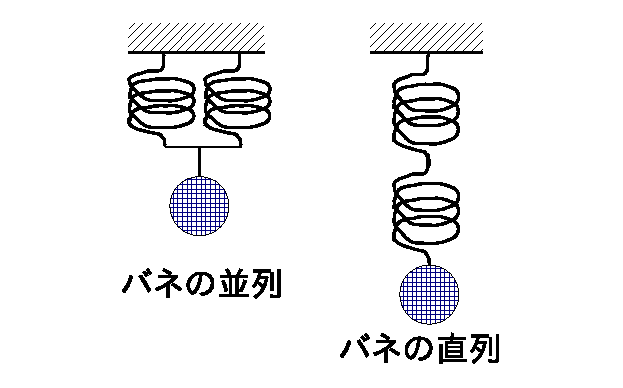
\includegraphics[width=7cm]{spring_serial.eps}
    \caption{バネの並列と直列}\label{fig:spring_serial}
\end{figure}
\end{q}

%
\begin{q}\label{q:spring_big}
バネ定数$k$のバネを$a$本だけ縦につないだものを$b$本だけ束ねて
大きなバネを作ると, そのバネ定数は$bk/a$となることを示せ。ヒント:
$n$本の直列を$m$本だけ並列。
\end{q}
\mv


断面積$A$, 長さ$L$の棒Xのバネ定数を考える。この棒を, 無数の小さい
(細くて短い)棒の集合(それぞれが弾性体)と考えれば, 棒Xの断面積は, 
小さい棒の並列の本数に, 棒Xの長さは, 小さい棒の直列の本数に, それぞれ比例
するので, 棒Xのバネ定数$k$は, $A/L$に比例する。そこで, 
\begin{eqnarray}
k=E\frac{A}{L}
\end{eqnarray}
と書く。このとき$E$を\textgt{ヤング率}\index{やんぐりつ@ヤング率}と呼ぶ。
ヤング率は物質に固有の定数(物性値)である。

\begin{q}\label{q:YoungModulus} 
\begin{enumerate}
\item ヤング率のSI単位は?
\item 鉄のヤング率を調べよ(「理科年表」\footnote{国立天文台(編)「理科年表」丸善。
毎年, 最新版が出ているが, 基本的なデータはそんなに頻繁には変わらないので, 昔の年のものを参照しても大丈夫。}などを使え)。
\item 長さ10~m, 直径2.0~mmの鉄線の先に10~kgの物体を吊り下げると, 鉄線はどのくらい伸びるか?
\item (3)で直径を半分(1.0~mm)にするとどうなるか?
\item (3)で鉄のかわりに銅を使うとどうなるか?
\end{enumerate}
\end{q}
\mv

ヤング率を使うと, フックの法則は以下のように書ける:
\begin{eqnarray}
F=-E\frac{A}{L}x
\end{eqnarray}
従って, 
\begin{eqnarray}
\frac{F}{A}=-E\frac{x}{L}
\end{eqnarray}
左辺の$F/A$は単位面積あたりの力で, 以前述べたように
「\textgt{応力}」\index{おうりょく@応力}と呼ぶ。「圧力」と呼んでもよさそうなもの
だが, この手の話題では圧力ではなく応力という言葉を使う。

右辺の$x/L$は単位長さあたりの伸びであり, 
「\textgt{ひずみ}」\index{ひずみ@ひずみ}と呼ぶ。応力を$\sigma$, 
ひずみを$\epsilon$と書くと, 上の式は, 
\begin{eqnarray}
\sigma=E\epsilon
\end{eqnarray}
と書ける(符号はとりあえず無視した)。これもフックの法則のひとつの表現である。
ここで示したフックの法則は, 1方向の伸びと, それと同方向のひずみとの間の関係で
あったが, それ以外にも, 様々な方向の応力と様々な方向の歪みに関しても同様の
関係が成り立つ。それを総称してフックの法則と呼ぶ。ただし, それをきちんと
表現するには, テンソル\index{てんそる@テンソル}という数学(「行列」の拡張版
みたいなもの)が必要であり, それは2年生以降に学ぶ。\mv

\begin{q}\label{q:stress_strain} 
\begin{enumerate}
\item 応力のSI単位は?
\item ひずみのSI単位は?
\end{enumerate}
\end{q}\mv


\begin{faq}{\small\textgt{フックの法則はバネだけの話かと
思っていましたが, もっと一般的なものなんですね。}
... そう。要するに力と変形の線型近似ですから, 
ほとんどの物体に成り立ちます。地震の波もフックの法則
で説明されます。}\end{faq}
\hv



\section{垂直抗力}
君が地面に立つとき, 君は地球から重力(引力)を受ける。
ところが, 君が静止しているためには, 君にかかる合力はゼロでなければ
ならない。さもなければ君の体は地面にどんどんめり込んでいくはずだ。
「力がどうであれ, そこに固い地面があれば, めり込んでいくわけがないだろう」
と君は思うかもしれない。しかし, その考え方は物理学ではダメなのだ。
物理学には「固いものにめり込んでいくことはできない」というような法則は
存在しない。固いものの表面で物体が静止することも, あくまで「力のつりあい」
で説明しなければならないし, 説明できるものなのだ。

君の足下に, 固い岩があったとしよう。その岩は, 君の体重のせいで, 
ごくわずかだが, 変形するのだ。その変形をもとに戻そうとする力, 
つまり弾性力が, 君の体を押し返すのだ。それが重力と釣り合って, 
君の体にかかる合力はゼロになり, 君は地上で静止できるのだ。

このように, 物体が, 固い面に対して垂直に力をかけると, 面はほとんど
変形せずに(といっても弾性力を発揮する程度には変形するが), それと
等しい大きさで逆向きの力を, 面は物体に対して働く。その力を
\textgt{垂直抗力}\index{すいちょくこうりょく@垂直抗力}と呼び, 慣習的に$N$で表す。

これは物体と「固い面」との間の「作用・反作用の法則」にすぎないじゃないか, 
と君は思うかもしれない。それは早計である。仮に垂直抗力が無くたって, 
作用・反作用の法則は成り立つ。君の体に働く重力は, 地球が君を引っ張るので
あり, その反作用として君は地球を引っ張る。君の足元に地面があったとしても, 
その地面がゆるゆるの状態で, 君を全く支えてくれないならば, 君の体は
加速度を持って地中に沈んでいくだけだ。それでも作用・反作用の法則は
(君の体と地球との間で)成り立っている。

でも, もしそこに固い地面があるならば, その地面が垂直抗力を発揮して君の
体を支えるのである。逆に言えば, 垂直抗力を発揮してくれるような面の
ことを「固い面」と言うのだ\footnote{この例では, 君の体に働く力は, 
地球から受ける重力と, 固い地面から受ける垂直抗力である。これらの釣り合い
によって君の体は静止する。一方, 固い地面(のごく表層)に働く力は, 君の体に
働く垂直抗力の反作用と, より下の地面から受ける弾性力である。これらの
釣り合いによって, 地面も静止する。}。

これらを総合して, 以下のような例を考えよう。図\ref{fig:slope}のように, 
傾斜角$\theta$のなめらかな斜面に, 質量$m$の物体が載っている。この物体には, 
重力$mg$が鉛直下向きに働いている。
\begin{figure}[h]
    \centering
    \includegraphics[width=7cm]{slope.eps}
    \caption{斜面に載った物体と, それにかかる重力}\label{fig:slope}

    \centering
    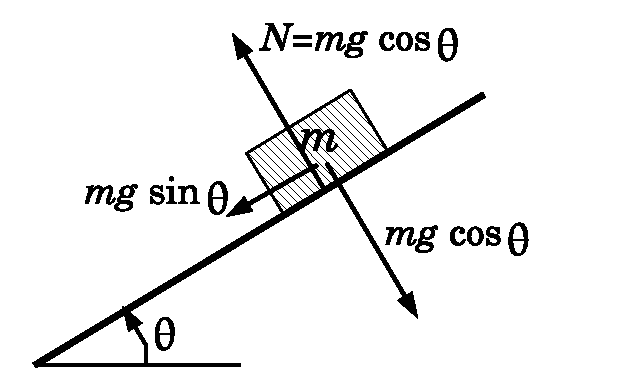
\includegraphics[width=7cm]{slope2.eps}
    \caption{物体は斜面から垂直抗力$N$を受ける。}\label{fig:slope2}

    \centering
    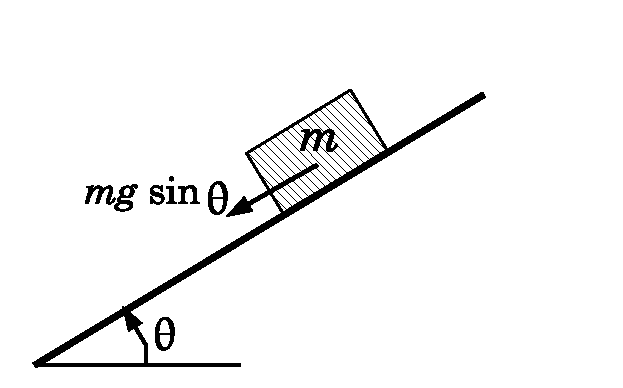
\includegraphics[width=7cm]{slope3.eps}
    \caption{結局, 物体は斜面に平行な力だけを受ける。}\label{fig:slope3}
\end{figure}

このとき, 図\ref{fig:slope}のように, 鉛直下向きの重力$mg$は, 斜面に沿った方向
の力と斜面垂直方向の力に分解して考えてもよい。前者の大きさは$mg\sin\theta$, 
後者の大きさは$mg\cos\theta$である。

と言われても, なぜ, 斜面に沿った方向と斜面垂直方向に分解するのだろうか?
そうするのが便利だからだ。というのも, もし斜面が固ければ, 物体が
動き得るのは斜面に平行な向きだけで, 斜面に垂直な方向には動けない。
従って, 斜面に垂直な方向では, 物体に働く力は釣り合っているはずだ。
それをまずあぶり出せば, 物体にかかる合力は求めやすくなる。

さて話を戻すと, 物体にはもともと重力の斜面垂直成分($mg\cos\theta$)
が働いているから, それと同じ大きさで物体を斜面に垂直に押し返す
垂直抗力$N$があるはずだ(図\ref{fig:slope2})。
一方, 今考えている斜面はなめらかなので, 斜面に沿った方向には斜面は物体に力を
およぼさない(つるつるしている!)。結局, 物体に働く重力と斜面から物体が受ける
垂直抗力を足し合わせると, 物体に働く力として, 図\ref{fig:slope3}のように, 
斜面に沿った重力$mg \sin \theta$だけを考えればよいことになる。

%
\begin{q}\label{q:force_rope2}
図\ref{fig:slope4}のように, 傾斜角30度と60度の2つのなめらかな斜面に, 
それぞれ質量3~kgと質量$m$の物体が載せられ, 滑車を介してロープでつながり, 静止している。
物体と斜面の間の摩擦は無く, 滑車とロープの間にも摩擦は無く, ロープの質量は
無視できるほど軽いとする。$m$を求めよ。ヒント:ロープにかかる張力の大きさ
を$T$とする。まず左の物体が静止する条件から$T$の大きさが求まる。そしてその$T$は, 
右の物体にもかかる。
\begin{figure}[h]
    \centering
    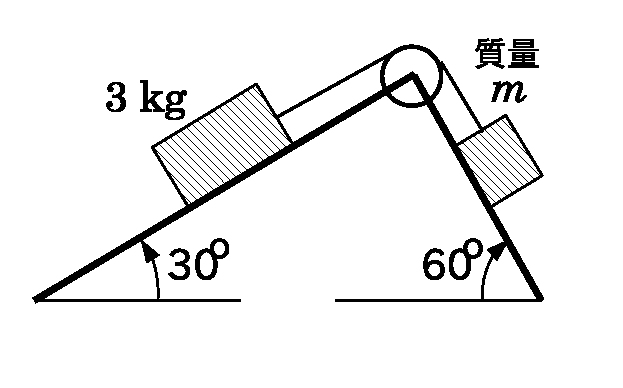
\includegraphics[width=7cm]{slope4.eps}
    \caption{2つの斜面に載せられ, ロープでつながって静止する2つの物体}\label{fig:slope4}
\end{figure}
\end{q}\mv

\begin{faq}{\small\textgt{斜面と滑車の問題は, 高校時代に挫折したとこです。}
... 滑車を介したロープはどこでも張力が同じ, というのがポイントです。}\end{faq}
\hv



\section{摩擦力(クーロンの摩擦法則)}

我々は日常経験から, 物体と物体を接触させたまま動かす(ずらす)
には力が必要だと知っている。ということは, 接触する物体どうしには, それらを
「ずらすまい」とする力が働くのだろう。そのような力を, \textgt{摩擦力}\index{まさつりょく@摩擦力}
という。これは, 以下の2つの式で表現されることが多い。

まず, $N$を, 物体どうしが接触面を介して接触面に対して垂直に互いに押し合う力とする。
2つの物体が相対的に静止している場合(ずれない場合)は, 摩擦力$F_{\text s}$は, 
\begin{eqnarray}
F_{\text s} \leq \mu N\label{eq:friction_s}
\end{eqnarray}
となる。また, 接触面を介して2つの物体が相対的に運動している場合
(ずれる場合)は, 摩擦力$F_{\text m}$は, 
\begin{eqnarray}
F_{\text m}=\mu' N\label{eq:friction_m}
\end{eqnarray}
となる。$F_{\text s}$を\textgt{静止摩擦力}\index{せいしまさつりょく@静止摩擦力}, 
$F_{\text m}$を\textgt{動摩擦力}\index{どうまさつりょく@動摩擦力}という。
また, $\mu, \mu'$は, それぞれ\textgt{静止摩擦係数}\index{せいしまさつけいすう@静止摩擦係数}, 
\textgt{動摩擦係数}\index{どうまさつけいすう@動摩擦係数}
とよばれる定数で, 接触面の物質や状態に依存する。

これを, \textgt{クーロンの摩擦法則}\index{くーろんのまさつほうそく@クーロンの摩擦法則}
という。この「クーロン」は電気的な力の「クーロン力」のクーロンさんと同一人物である。
偉い学者は一人でいくつもの法則を発見するので, 後世の我々は
「クーロンの法則といってもどの法則だ?」と混乱してしまうのだが, まあそれは仕方がない。

さて, 式(\ref{eq:friction_s})に不等号"$\leq$"が入っているのは, 次のような理由
による:摩擦力は, 接触中の2つの物体を「ずらすまい」とする力である。従って, 
静止中の2つの物体の間に, 互いをずらそうとする力がそもそも働いていない場合は, 
あえて「ずらすまい」とする必要はない。そのとき, 静止摩擦力はゼロであるべきだ。
また, たとえ, 「ずらそうとする力」が働いても, それが弱ければ, それを打ち消す
程度の摩擦力があれば十分であり, それ以上は必要ない。
物体が静止しているからには「力のつりあい」が成り立つはずで, となると静止摩擦力は
「ずらそうとする力」と反対の向きに\textgt{同じ大きさで}働いていると考えざるを得ないのだ。
従って, 静止摩擦力は, 
ある一定の範囲($\mu N$以下)で, 「ずらそうとする力」に対応してそれを
"ちょうど"打ち消す力を発揮するのである。

さて, 多くの場合, $\mu'<\mu$である。つまり静止摩擦係数$\mu$は動摩擦係数$\mu'$より
大きい。つまり, 摩擦力は, 静止状態の方が, 動いている状態よりも強い。
それがなぜなのかは, 様々な説があるが, 決定打は無い。

この「クーロンの摩擦法則」も, 一般性の低い「しょぼい」法則である。
単なる経験則であり, この法則から外れるような例もある。摩擦力は, 結局, 
物質と物質の間に働く力なので, おそらく電気力がその根源なのだろう。しかし, 
基本法則からクーロンの摩擦法則を導くことには, まだ誰も成功していない。実は, 
摩擦力の起源や実体は, よくわかっていないのだ。クーロンの摩擦法則は誰もが
「しょぼい」と思っているが, 誰もそれに代わる法則を見つけ出せないでいる...\mv

\begin{faq}{\small\textgt{$\mu' < \mu$となる理由がわかりません。}
... 正確な理由は不明。よく言われるのが, 静止状態では接触面での微妙な凹凸が互いにかみ合って
抵抗が大きいのに対し, 動いているとなかなか凹凸がかみあわず, 滑りやすくなる, という説明。}\end{faq}\mv

\begin{faq}{\small\textgt{「車のブレーキは, タイヤを完全に止めるより, 
少し回しながらのほうが, 地面との摩擦が大きくなって早く止まれる」と
聞いたことがあります。$\mu'<\mu$と関係していますか?}
... まさにそうです。それを利用したのがABS (アンチロック・ブレーキング・システム)です。}\end{faq}\mv


\begin{q}\label{q:friction} 
\begin{enumerate}
\item クーロンの摩擦法則とは何か?
\item 摩擦係数とは何か?
\item 摩擦係数の次元は?
\item アンチロック・ブレーキング・システムを説明せよ。
\end{enumerate}
\end{q}
\mv

\begin{q}\label{q:friction_slope}
傾斜角$\phi$の斜面に, 質量$m$の物体が載って, ぎりぎりで静止している。
これよりも少しでも傾斜がきつければ, 物体は滑り出してしまう。このとき, 傾斜角$\phi$
と静止摩擦係数$\mu$の間に, 次の関係が成り立つことを示せ(このような$\phi$を
\textgt{安息角}という)。
\begin{eqnarray}
\mu=\tan \phi
\end{eqnarray}
\end{q}
\mv

\begin{q}\label{q:slope_spring_friction}
図\ref{fig:slope_spring_friction}のように, 摩擦のある斜面(静止摩擦係数$\mu$)
の上方からバネ(バネ定数$k$)で物体(質量$m$)が吊られて静止している。そのような
状態が実現できるようなバネの伸び縮みの範囲を求めよ。
\begin{figure}[h]
    \centering
    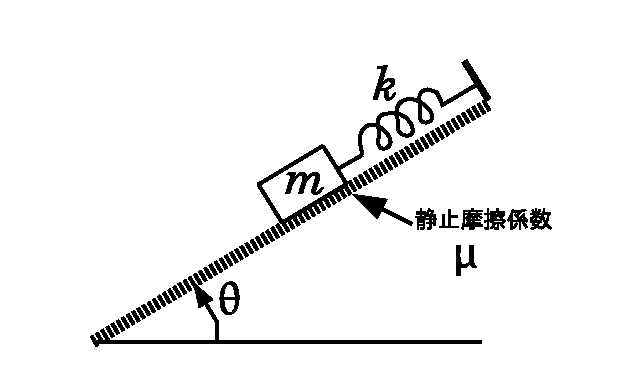
\includegraphics[width=7cm]{slope_spring_friction.eps}
    \caption{摩擦のある斜面に, バネで吊るされた物体}\label{fig:slope_spring_friction}
\end{figure}
\end{q}
\hv


\section{系とは何か?}

これまで扱った多くの例や問題では, それぞれで, 単純化された状況を考えてきた。
例えば図\ref{fig:slope_spring_friction}では, ひとつの斜面と
その上でバネにつながって静止する物体, そしてそれに働く重力\textgt{だけ}を考えた。
実際は世界にはもっとたくさんの物体があるしたくさんの斜面があるしたくさんの力
がある。バネにつながって静止した物体に, 突然上空から隕石が落ちてきて衝突
する可能性も0ではないのだ。

しかし, 科学をやるときは, 世界の中のごく一部だけを
限定的に切り出して単純化し, それ以外のすべてのものを無視した状況を設定する
ことがよくある。そういう状況設定を「\underline{系}」\index{けい@系}
(system)という。それは, 言ってみれば, 当面の問題や議論のためだけ
に極限まで単純化された「世界のモデル」である。例えば, 2つの物体しかない
世界や, バネにつながった物体が斜面に載っている以外には何も無い世界
を考えるのだ。それが系である。

系という言葉は, 本書では今後, たくさん出てくるし, 化学などでもよく出てくるので, 
よく理解しておこう!\mv

\begin{q}\label{q:whatissystem} 系とは何か?\end{q}
\hv




\begin{faq}{\small\textgt{黒板を手で押すとき, 黒板がわずかに
変形してその弾性力が手を押し返すことで手が静止する
と聞きました。でも, 手と黒板の間に, もし作用・反作用の法則がはたらくなら, 黒板は変形
しないでも, 同じ大きさで逆向きの力が手にはたらくと思います。大きさが同じなら釣り合うん
じゃないんですか?}
... とても良い質問です。作用・反作用の法則を学ぶとき, 多くの人が感じる疑問です。
物体が動く(運動状態を変える)かどうかは, 「その物体に働く力」
が釣り合っているかどうかで決まります。ところが作用・反作用
の法則は, 「その物体に働く力」と同じ大きさで逆向きに「相手の物体に働く力」があるという話です。
なので, 「大きさが同じで向きが逆」ということだけを切り出して「ならば力は釣り合うのでは?」
と考えるのは早計です。手が物体を押す力と, 物体が手を押し返す力が「釣り合っている」としても, 
そのことは物体の運動にも手の運動にも, 直接的には無関係なのです。
つまり, 作用・反作用の法則と力のつりあいは無関係なのです。

例として, ボール投げを考えましょう。ボール投げの際, 手はボールに力をかけますが, 
その力はボールを加速することに寄与します(これは後に学ぶ運動方程式で説明
されます)。一方, ボールは等しい大きさで逆向きに手を押し返します(作用・反作用の法則)。
だからボールを投げるときに手は負担を感じるのです(だからピッチャーには体力が必要)。
このとき, ボールにかかる力は釣り合っていません。手にかかる力(ボールから受ける反作用の
力と, 腕の筋肉が手を押す力)も釣り合っていません。

手が黒板を押すとやがて動かなくなるのは, 筋肉(それは肩から手首にかけての部分)
が手(手首から先の部分)を押そうとする力と, 黒板が弾性力(それは結局は垂直抗力)で手
を押そうとする力が釣り合うからです。その弾性力は, 黒板がわずかだけど歪むことで
発生します。従って, 手が黒板を押し始めてから黒板が十分に歪むまでの間は, 黒板の弾性力
は手が押す力よりも弱いので, 黒板は徐々に押し込まれて変形します。その過程では, 
手が押す力の「余り」は, 黒板の変形を加速することに寄与します(運動方程式)。
そして, それらの和, つまり手が押す力と同じ大きさで逆向きの力を手は黒板から
受けます(これが作用・反作用の法則)。これは変形の途中でも, 変形しきったときでも, 
同じこと。ところが変形しきったときは, 黒板の加速度はゼロになるので, 
結局, 手が押す力と黒板の弾性力は等しい大きさになります。}\end{faq}

\begin{faq}{\small\textgt{物体に力がかかるとき, ごくわずかでも
めり込むなら, かなり長い時間, 力をかけていたら, その物体はへこみますか?}
... 力の大きさと素材によりますが, そういう場合も多いでしょう。
短時間では弾性的な(変形に比例した反発力を生じ, 力が取り除かれると
元に戻る)物体も, 長時間, それなりの力にさらされ続けたら, 反発力
を徐々に失い, 変形が戻らなくなったりします。この性質を弾塑性と
呼びます。「レオロジー」という学問分野で扱います。}\end{faq}
\hv

\begin{exq} 質量1~gの物体を1~cm~s$^{-2}$の加速度で動かす力の大きさを1~dynという
(dynはダインと読む)。0.03~Nをdyn単位で書き換えよ。\end{exq}

\begin{exq} 1枚のティッシュペーパーから, 幅2cmほどの帯を2枚切り出し, それぞれ帯Aと帯Bと
呼ぶ。帯Aはそのままにし, 帯Bはねじる(数10回)。それぞれの帯について両端をひっぱって
引きちぎる。どちらが切れにくい(引きちぎるのにより大きな力が必要)か? その理由とともに
述べよ。\end{exq}

\begin{exq} 質量2.0~kgの質点に, 3.0~Nの力をかける。質点に生じる加速度の大きさを求めよ。
ただし基本法則に基づいて根拠もきちんと述べること。\end{exq}

\begin{exq} バネ定数2.0~N/mのバネを, 左端から1.0~N, 右端から1.0~Nの力で
それぞれ引っ張った。伸びはどのくらいか?\end{exq}


%\section{圧力}

%\section{浮力}


\section{解答}

% 自然界に存在する, 根源的な4つの力とは何か?
\noindent{\textbf{答}}\ref{q:4forece} 重力・電磁気力・強い力・弱い力
\mv

% 万有引力定数を$G=6.7 \times 10^{-11}$ N~m $^2$kg$^{-2}$, 地球の半径を$r=6400$ km,
\noindent{\textbf{答}}\ref{q:grav_accel}\\
略。ヒント: \eref{eq:gravity_univ}に適切に値を代入して計算すればよい。ただし, $r$はkmで与えられて
いるので, mに換算すること。つまり, $r=6.4\times10^6$~mとすること。
\vspace{0.2cm}

%\noindent{\textbf{答}}\ref{q:weight_calib} 略。
%\vspace{0.2cm}

% 重力加速度とは何か?
\noindent{\textbf{答}}\ref{q:what_is_g}\\
地表付近にある質量$m$の物体が地球から受ける重力は$mg$
と書ける。このときの定数$g$が重力加速度
\footnote{たまに, 重力加速度とは$GM/r^2$である, という人がいるが, 
間違い。なぜなら, この式は, 地球を静止した完全な球体とみなしており, 
この式に従えば地表のどこでも同じ値になってしまうから。実際の$g$の値は, 
場所によって微妙に異なる。例えば地下に重いものがある場合は, その直上の地表付近では
$g$は大きくなる。低緯度では地球の自転による遠心力(後に学びます)の影響も$g$の
値に入って来る。}。
%また, ウィキペディアなどには「地球表面付近において物体が
%受ける重力の加速度」が重力加速度であると書かれていますが, これもダメです。
%「重力の加速度」とは何か? 重力が加速されるのか? 重力によって何かが加速される
%のか? 地面に置いてある石は重力を受けるけど, 加速されてませんよね?}。
\vspace{0.2cm}

% 高度36000 kmの上空を飛ぶ静止衛星には, 地表での重力の何パーセントの重力がかかるか? 
\noindent{\textbf{答}}\ref{q:geostat_sat}\\
地球中心から地表までの距離を$r_1$, 地球中心から旅客機または静止衛星
までの距離を$r_2$とする。質量$m$の旅客機または衛星が仮に地表にあるときの重力を$F_1$, 
それらが上空にあるときの重力を$F_2$とすると, 
\eref{eq:gravity_univ}より, 
\begin{eqnarray*}
&&F_1=G\frac{Mm}{r_1^2},\quad\quad
F_2=G\frac{Mm}{r_2^2}, \quad\quad\text{従って,}\\
&&\frac{F_2}{F_1}=\frac{r_1^2}{r_2^2}=\Bigl(\frac{6400 \text{km}}{r_2}\Bigr)^2\quad\text{である。}
\end{eqnarray*}
旅客機の場合, $r_2=$6,400~km+10,000~m=6,410~kmを上の式に代入すると, 0.9969$\cdots$。
従って地表での重力の99.7パーセント(ほぼ100パーセント)。静止衛星の場合は, 
$r_2=$(6400~km)+(36000~km)$\fallingdotseq42000$~kmを上の式に代入すると, 0.023$\cdots$。
従って, 地表での重力の約2パーセント。
\mv

% 月の質量は地球の質量の1/80, 月の半径は
\noindent{\textbf{答}}\ref{q:moon_gravity} 地球の半径を$r_1$, 月の半径を$r_2$, 地球の質量を$M_1$, 月の質量を$M_2$とする。
さて, 質量$m$の物体が地表にあるとき地球からうける重力を$F_1$, 月の表面にあるとき月から
うける重力を$F_2$とすると, \eref{eq:gravity_univ}より, 
\begin{eqnarray*}
&&F_1=G\frac{M_1m}{r_1^2},\quad,\quad
F_2=G\frac{M_2m}{r_2^2}\quad\quad\text{従って,}\\
&&\frac{F_2}{F_1}=\frac{M_2}{M_1}\times\Bigl(\frac{r_1}{r_2}\Bigr)^2
\end{eqnarray*}
$M_2/M_1=1/81.3$, $r_2/r_1=1/3.68$を代入すると,
\begin{eqnarray}
\frac{F_2}{F_1}=\frac{1}{81.3}\times3.68^2=\frac{1}{6.00}
\end{eqnarray}
従って, 1/6倍。
\mv

% 地表での平均的な大気圧は, 1000hPa程度であ
%\noindent{\textbf{答}}\ref{q:atm_pressure} 1.0~m$^2$の地表面の上空にある大気の質量を$m$とし, それにかかる重力を$F$とする。
%$F=mg=1000\times10^2$~Pa$\times 1$~m$^2$=$10^5$~N。従って, 
%\begin{eqnarray}
%m=\frac{F}{g}=\frac{10^5\text{ N}}{9.8\text{ m s}^{-2}}\fallingdotseq10^4\text{ kg}
%\end{eqnarray}
%\mv

% クーロンの法則とは何か?
\noindent{\textbf{答}}\ref{q:coulomb_law} 電荷$q_1$と電荷$q_2$をそれぞれ持つ粒子が距離$r$だけ離れて静止して
いれば, その間に, 以下の式であらわされる力$F$が生じる:
\begin{eqnarray*}
F=k\frac{q_1 q_2}{r^2}
\end{eqnarray*}
($k$は定数で, $k=8.987\cdots\times 10^{9}$~N~m$^2$~C$^{-2}$である。)
これを, クーロンの法則と呼ぶ。
\mv

% 電荷素量とは何か?
\noindent{\textbf{答}}\ref{q:element_charge} 電子や陽子が持つ電荷の大きさ(ただし符号を考えない)。$q_e=1.602\times10^{-19}\text{ C}$。
\vspace{0.2cm}

% 互いに1m離れたところに存在する2個の電子の間
\noindent{\textbf{答}}\ref{q:elec_grav_compare}
\begin{enumerate}
\item \eref{eq:coulomb}より, 
\begin{eqnarray}
F_e&=&8.987\times 10^{9}\text{~N~m$^2$~C$^{-2}$}\times\frac{(1.602\times10^{-19}\text{ C})^2}{(1\text{ m})^2}\nonumber\\
   &=&2.3\times10^{-28}\,\, \text{N}
\end{eqnarray}
\item \eref{eq:gravity_univ}より, 
\begin{eqnarray}
F_g&=&6.7 \times 10^{-11}\text{ N m}^2{\text kg}^{-2}
\times\frac{(9.1\times10^{−31}\text{ kg})^2}{(1\text{ m})^2}\nonumber\\
&=&5.5\times10^{-71}\,\, \text{N}
\end{eqnarray}
\item
\begin{eqnarray}
\frac{F_g}{F_e}=2.4\times10^{-43}
\end{eqnarray}
注: このように, クーロン力は重力よりもはるかに大きい。
米国の物理学者リチャード・ファインマンは, 
これを, 「光が陽子1個の端から端まで通り過ぎるのにかかる
時間と, 宇宙の年齢との違いくらい大きい」と表現している。
\end{enumerate}
\vspace{0.2cm}

\noindent{\textbf{答}}\ref{q:Coulomb_EF} その場所に電荷$q$の荷電粒子を
置くと, かかる力の大きさ$F$は, 
\eref{eq:coulomb}より, 
\begin{eqnarray}
F=\frac{k\,q_{\text{e}}\,q}{r^2}
\end{eqnarray}
ここで, $q_{\text{e}}=1.602\times10^{-19}$~C
は電荷素量, $r=1$~m, $k=8.987\times 10^{9}$~N~m$^2$~C$^{-2}$。
電場の大きさは$F/q$だから, 
\begin{eqnarray}
\frac{F}{q}=\frac{k\,q_{\text{e}}\,q}{r^2\,q}=\frac{k\,q_{\text{e}}}{r^2}
\end{eqnarray}
これを計算すると, $1.44\times10^{-9}$~N/C。\mv


% 片端が壁にとりつけられた綱を
\noindent{\textbf{答}}\ref{q:force_rope1}\\
「人対壁」では, 人Aがロープを引く力は, ロープの各箇所で断面の左側に
大きさ$F$で右向きにかかる。その反作用は, 各断面の右側に大きさ$F$で左向きにかかる
(これが張力)。それがロープの左端(壁との接点)まで伝わり, 壁との接点では, 
壁はロープから, 大きさ$F$で右向きの力を受ける。その反作用として, ロープは壁
から大きさ$F$で左向きの力を受ける(この「壁が引く力」がロープの各箇所での
左向きの力の源泉であり, そのおかげで「作用・反作用の法則」とつじつまが合う)。
これは, 壁のかわりに別の人がロープを左端で大きさ$F$の力で左向きにひっぱるのと
同じこと。従って, 「人対人」でも, 「人対壁」でも同じことになる。
\vspace{0.2cm}

%
\noindent{\textbf{答}}\ref{q:force_rope3}\\
君の体には2箇所でロープから上向きにひっぱられている。また, ロープの張力$T$は, 
ロープのどこでも等しい。従って, 君の体には上向きに$2T$の力がかかる。一方, 
重力によって, 君の体に下向きに$mg$の力がかかる。座標軸を, 上向きを正にとると, 力のつりあいから, 
$2T-mg=0$。従って, $T=mg/2$。一方, 君の手がロープを引く力は$T$に等しいので, 
結局, $mg/2$に等しい。
\mv

%
\noindent{\textbf{答}}\ref{q:force_rope4}\\
滑車Bの両端のそれぞれで, ロープの張力$T$が滑車Bを上向きに引く。一方, 
滑車Bには質量$m$の物質にかかる重力$mg$が下向きにかかる。力のつりあい
から, $2T-mg=0$。従って$T=mg/2$。ロープの張力は, ロープのどこでも
等しいから, 君の手にかかる力も$T$, すなわち$mg/2$である。
\vspace{0.2cm}

%
\noindent{\textbf{答}}\ref{q:force_rope5}\\
君の手がロープを引く力は, 君の手の筋肉の筋繊維の収縮から生じる。
この現象は, 筋繊維を構成する高分子の変形によって生じる。分子スケール
の現象を支配する力は, ほとんどの場合, 電気力である。従って, 君の手が
ロープを引く力の根源は電気力である。
\vspace{0.2cm}

%
\noindent{\textbf{答}}\ref{q:Hooke_law}
\begin{enumerate}
\item バネの伸び(変位)$x$と, バネが押す力$F$が比例する, という法則。
\item フックの法則を$F=-kx$と書くときの係数$k$。
\item $k=-F/x$なので, $F$の単位(すなわちN=kg~m~s$^{-2}$)を$x$の
単位(すなわちm)で割ればよい。答は, kg~s$^{-2}$。
\end{enumerate}
\vspace{0.2cm}

\noindent{\textbf{答}}\ref{q:elasticity}\\
力と変位が比例する, という, フックの法則が成り立つような力を
弾性力という。弾性力だけで変形する物体を弾性体という。
\vspace{0.2cm}

\noindent{\textbf{答}}\ref{q:plasticity}\\
塑性体とは, 変形すると元に戻らない物体である。(弾性体は, 
力がかかると変形するが, かかる力が無くなれば元にもどる。)
\vspace{0.2cm}

\noindent{\textbf{答}}\ref{q:spring_moon}\\
質量$m$の物体が地表にあるとき, バネの伸びが$x_0$だったとする。
バネの弾性力と(地球からの)重力のつりあいは次式になる:
\begin{eqnarray}-kx_0+mg=0\end{eqnarray}
一方, 質量$m$の物体が月面にあるとき, バネの伸びが$x_1$だったとする。
月面での(月から受ける)重力は, 問\ref{q:moon_gravity}より, 地表での(地球から受ける)重力の約1/6
なので, バネの弾性力と(月からの)重力のつりあいは次式になる:
\begin{eqnarray}-kx_1+mg/6=0\end{eqnarray}
この2つの式から$mg$を消去すれば, 
\begin{eqnarray}kx_1=kx_0/6\end{eqnarray}
従って, $x_1=x_0/6$。従って, 月面でのバネの伸びは, 地表での約1/6倍。
\vspace{0.2cm}

\noindent{\textbf{答}}\ref{q:spring_double_parallel}\\
下向きに座標系をとる。左側のバネをA, 右側のバネをBと呼ぶ。
バネAについて, バネが下端に働く力を$F$, 伸びを$x$とすると, フックの法則より, 
\begin{eqnarray}F=-kx\end{eqnarray}
である。左右対称なので, まったく同じ式が, バネBについても成り立つ。
一方, 質量$M$の物体にかかる力は, 2つのバネから受ける力, つまり$2F$と, 
重力$Mg$である。物体が静止するには合力はゼロだから, 
\begin{eqnarray}2F+Mg=0\end{eqnarray}
これらの式から$F$を消去すると, 
\begin{eqnarray}-2kx+Mg=0\end{eqnarray}
従って, 
\begin{eqnarray}x=\frac{Mg}{2k}\end{eqnarray}
である。バネが1本だけのときは, $x=Mg/k$なので(\eref{eq:x_mg_k}), この
結果は, $k$が2倍になったとみなせる。
\vspace{0.2cm}

\noindent{\textbf{答}}\ref{q:spring_double_series}\\
下向きに座標系をとる。上のバネをC, 下のバネをDと呼ぶ。
バネCについて, バネが下端に働く力を$F_1$, 伸びを$x_1$とすると, フックの法則より, 
\begin{eqnarray}F_1=-kx_1\end{eqnarray}
である。バネDについても同様に, バネが下端に働く力を$F_2$, 伸びを$x_2$とすると, 
フックの法則より, 
\begin{eqnarray}F_2=-kx_2\end{eqnarray}
である。一方, 質量$M$の物体にかかる力は, バネDが下端に働く力, つまり$F_2$と, 
重力$Mg$である。物体が静止するには合力はゼロだから(力のつりあい), 
\begin{eqnarray}F_2+Mg=0\end{eqnarray}
である。また, バネDにかかる力は, バネCが下端に働く力$F_1$と, 物体がバネDを引っ張る
力(つまり重力)である。バネDに関する力のつりあいから, 
\begin{eqnarray}F_1+Mg=0\end{eqnarray}
これらの式から, 
\begin{eqnarray}Mg=-F_1=-F_2=kx_1=kx_2\end{eqnarray}
従って, 
\begin{eqnarray}x_1=x_2=\frac{Mg}{k}\end{eqnarray}
である。2本のバネの伸びの合計$x$は, 
\begin{eqnarray}x=x_1+x_2=\frac{2Mg}{k}\end{eqnarray}
バネが1本だけのときは, $x=Mg/k$なので(\eref{eq:x_mg_k}), この
結果は, $k$が1/2倍になったとみなせる。
\vspace{0.2cm}

\noindent{\textbf{答}}\ref{q:spring_big}\\
問\ref{q:spring_double_series}と同様に考えれば, バネ定数$k$のバネを$a$本, 縦につなぐと, 
バネ定数は$k/a$となる。問\ref{q:spring_double_parallel}と同様に考えれば, バネ定数$k/a$のバネを$b$本, 
束ねる(並列につなぐ)と, バネ定数は$bk/a$となる。
\vspace{0.2cm}

\noindent{\textbf{答}}\ref{q:YoungModulus}\\
\begin{enumerate}
\item $E=kL/A$で, $k$のSI単位はkg~s$^{-2}$, $L/A$のSI単位はm/m$^{2}$=m$^{-1}$なので, $E$の単位は
kg~s$^{-2}$m$^{-1}$。順番を入れ替えてkg~m$^{-1}$~s$^{-2}$などでもOK。なんと! これはPa, すなわち
圧力のSI単位ではないか!
\item 約$2.0\times10^{11}$~Pa。
\item まずこの鉄線のバネ定数$k$を求める。$L=10$~m, $A=3.14\times(0.002\text{ m}/2)^2=3.1\times10^{-6}$~m$^2$。
従って, $k=EA/L=6.2\times10^{4}$~kg~s$^{-2}$。さて, 質量$m$の物体を吊り下げたときの伸び$x$は, 
\begin{eqnarray*}x=\frac{mg}{k}=\frac{10\text{ kg}\times9.8\text{ m s}^{-2}}{6.2\times10^4\text{ kg s}^{-2}}=1.6\times10^{-3}\text{ m}\end{eqnarray*}
従って, 1.6~mm (約2~mm) 伸びる。
\item 伸びはバネ定数に反比例する。バネ定数は断面積に比例する。従って, 伸びは断面積に反比例
する。従って, 直径を半分にすると断面積が1/4倍になり, 伸びは4倍になる。従って, 伸びは6.4~mmになる。
\item 銅のヤング率は$1.3\times 10^{11}$~Pa。鉄の約0.65倍。伸びはバネ定数に反比例し, バネ定数は
ヤング率に比例する。従って伸びはヤング率に反比例する。従ってヤング率が0.65倍になれば伸びは1/0.65倍。
従って, 2.5~mm程度になる。
\end{enumerate}
\vspace{0.2cm}

%
\noindent{\textbf{答}}\ref{q:stress_strain}
\begin{enumerate}
\item $\sigma=F/A$より, $\sigma$のSI単位は, kg~m~s$^{-2}$/m$^2$ =kg~m$^{-1}$s$^{-2}$=Pa。
\item $\epsilon=x/L$より, $\epsilon$の単位は, m/m=1。従って, 単位無し! (無次元)
\end{enumerate}
\vspace{0.2cm}

% 傾斜角30度と60度の2つのなめらかな斜面に, 
\noindent{\textbf{答}}\ref{q:force_rope2}\\
3~kgの物体にかかる重力の, 斜面平行方向の大きさは, $(3\text{ kg})\times g\times \sin (\pi/6)$。
質量$m$の物体にかかる, 斜面平行方向の力の大きさは, $mg\times \sin (\pi/3)$。これらは
ともにロープの張力と等しい。ロープの張力$T$は, ロープのどこでも等しいから, 
$T=(3\text{ kg}) g \sin (\pi/6)=mg \sin (\pi/3)$。従って, 
\begin{eqnarray}
m=\frac{(3\text{ kg})g\sin(\pi/6)}{g\sin(\pi/3)}=\sqrt{3}\text{ kg}\fallingdotseq 1.7\text{ kg}
\end{eqnarray}
\mv

%
\noindent{\textbf{答}}\ref{q:friction}
\begin{enumerate}
\item 物体どうしが接触している場合, 静止摩擦力$F_{\text s}$と動摩擦力$F_{\text m}$が, 
$F_{\text s} \leq \mu N, F_{\text m}=\mu' N$となること。ここで, $N$は物体どうしが
互いに接触面に垂直に押し合う力。$\mu, \mu'$は, それぞれ静止摩擦係数, 
動摩擦係数とよばれる定数。
\item クーロンの法則が上の式のようにかける時の, $\mu$や$\mu'$のこと。
\item $\mu'=F_{\text m}/N$であり, $F_{\text m}$も$N$も力なので, その比である$\mu'$は無次元。
$\mu$も同様に無次元。
%\item 略。
\end{enumerate}
\mv

\noindent{\textbf{答}}\ref{q:friction_slope}\\
質量$m$の物体に, 斜面に平行にかかる重力(重力の斜面成分)は$mg \sin \phi$。
これが静止摩擦力$F_{\text s}$とつりあっている。いま, 静止摩擦力は上限の状態なので, クーロンの
摩擦の法則より, $F_{\text s}=\mu N$。ここで$N$は物体と斜面の間に働く, 斜面に垂直方向の力で
あり, これは重力の斜面垂直成分に等しい:$N=mg\cos\phi$。従って, $F_{\text s}=\mu mg\cos\phi$。
斜面に平行な方向の力のつりあいより, $mg \sin \phi=F_{\text s}=\mu mg\cos\phi$。従って, 
\begin{eqnarray}\mu=\frac{mg\sin\phi}{mg\cos\phi}=\frac{\sin\phi}{\cos\phi}=\tan\phi\end{eqnarray}
\mv

\noindent{\textbf{答}}\ref{q:slope_spring_friction}\\
斜面に平行で上向き(上り坂方向)に$x$軸をとる。物体をとりつける前のバネの
自然長での末端位置を$x=0$とし, 物体をとりつけた後のバネの末端位置を$x$とする。
物体にかかる, 摩擦力以外の力は, 重力: $-mg\sin\theta$, 弾性力: $-kx$の
2つである。この合力が, 静止摩擦力$F_{\text s}$と釣り合うのだから, 
\begin{eqnarray}-mg\sin\theta-kx+F_{\text s}=0\end{eqnarray}
である。ここで, 垂直抗力は$mg\cos\theta$なので, 
$|F_{\text s}|\leq\mu mg\cos\theta$である。従って, 
\begin{eqnarray}|F_{\text s}|=|mg\sin\theta+kx|\leq\mu mg\cos\theta\end{eqnarray}
である。従って, 
\begin{eqnarray}-\mu mg\cos\theta\leq mg\sin\theta+kx\leq\mu mg\cos\theta\end{eqnarray}
である。従って, 
\begin{eqnarray*}-\mu mg\cos\theta-mg\sin\theta\leq kx\leq\mu mg\cos\theta-mg\sin\theta\end{eqnarray*}
である。従って, 
\begin{eqnarray*}\frac{mg}{k}(-\mu \cos\theta-\sin\theta)\leq x\leq\frac{mg}{k}(\mu \cos\theta-\sin\theta)\end{eqnarray*}\mv

%\noindent{\textbf{答}}\ref{q:whatissystem} 略。

\begin{faq}{\small\textgt{解答を省略するの, やめてください。} ... 
これ, すごく悩ましい話です。私は10年くらいかけて数学や物理学の授業テキストを作っていますが, 最初のころは問題の解答が雑だったり「略」が多かったのです。その頃は, 学生がよく「問題が解けません...」といって質問に来ました。そして問題を一緒に考えて, 単なる「正解」だけでなく, 学生の考え方の癖や, 勉強法などまでも, 助言できました。解答のついていない問題を友達と一緒に考えているうちに, 数学や物理学の楽しさにのめりこんでしまった, というタイプの学生もたくさんいました。

しかし, 学生から「ちゃんと解答をつけてください」と言われて, 丁寧に解答をつけるようにしたら, 学生は質問に来なくなりました。それで学力は伸びたかというと, そうでもありません。むしろ, 「単に正解を覚えて再現してるだけ」で, 深くは理解していない学生が増えました。

学問は, 「誰かが作った正解を覚えこむもの」ではなく, 自分の頭で納得するまで考えるものです。そこが苦しいところでもあり, 楽しいところでもあります。そしてそれは大学教育の最も大事な部分です。「問題の解答」は, そこにおいて, むしろ悪影響をもたらすものではないか, と, 私は悩んでいます。あなたはどう思いますか?}\end{faq}

\begin{faq}{\small\textgt{でも, 自力で解いた後の答え合わせには, 正解を教えてもらうことが必要です。} ... 
大学では「正解」は, 誰かが与えるものでなく, あなたが作るものです。いろんな観点から考えぬいて, 「これが正しい!」とあなた自身が納得し, 人にも説明できるなら, それが「正解」です。実際, 教員や教科書が与える「正解」には, 間違っていることも多いのですよ。お互いの「正解」を比べて議論しながら, 「より正しい正解」を作るのです。学問とは本来, そういうものです。}\end{faq}

\begin{faq}{\small\textgt{でも, 解答が無いと勉強の効率が悪いです。いくら考えてもわからないときは解答を見るしかありません} ... 
その気持ちわかります。私もそう思います。でもね。解答があると, 突き詰めて考える前にどうしても見たくなってしまうものです。あなたはそれを自制できるかもしれませんが, 「問題は正解を丸写しにして覚えるもの」と思っている人も多いのです。}\end{faq}

\begin{faq}{\small\textgt{じゃあ, どうすればいいのですか?} ... 
質問に来ればよいのです。あるいは, 友達同士で一緒に考えたり教え合えばよいのです。}\end{faq}

